%# -*- coding: utf-8 -*-
% !TeX encoding = UTF-8 Unicode
% !TeX spellcheck = en_US
% !TeX TS-program = xelatex
%~ \XeTeXinputencoding "UTF-8"
% vim:ts=4:sw=4
%
% 以上设定默认使用 XeLaTex 编译,并指定 Unicode 编码,供 TeXShop 自动识别

\chapter{High Level Design}



\begin{enumerate}
  \item 使用 flowchart 将处理流程初步理清
  \item 使用 \href{http://www.cascading.org/}{Cascading}/MapReduce 实现系统
  \item 测试
\end{enumerate}


\section{介绍}

\begin{enumerate}
  \item simulation task:
  generate the NS2 TCL scripts, and run ns2

  \item plotting figures:
  
\end{enumerate}


\section{整体结构}
图 \ref{fig:system} 是整个系统的运行框架。

\definecolor{vidtransoriginfile}{HTML}{D7FE39}
\definecolor{vidtranstmpfile}{HTML}{EDE80F}
\definecolor{vidtransfinalfile}{HTML}{FFE985}
\definecolor{vidtransprocess}{HTML}{FEA93E}
\definecolor{vidtransfuncio}{HTML}{DADAFF}
\begin{figure}\centering
  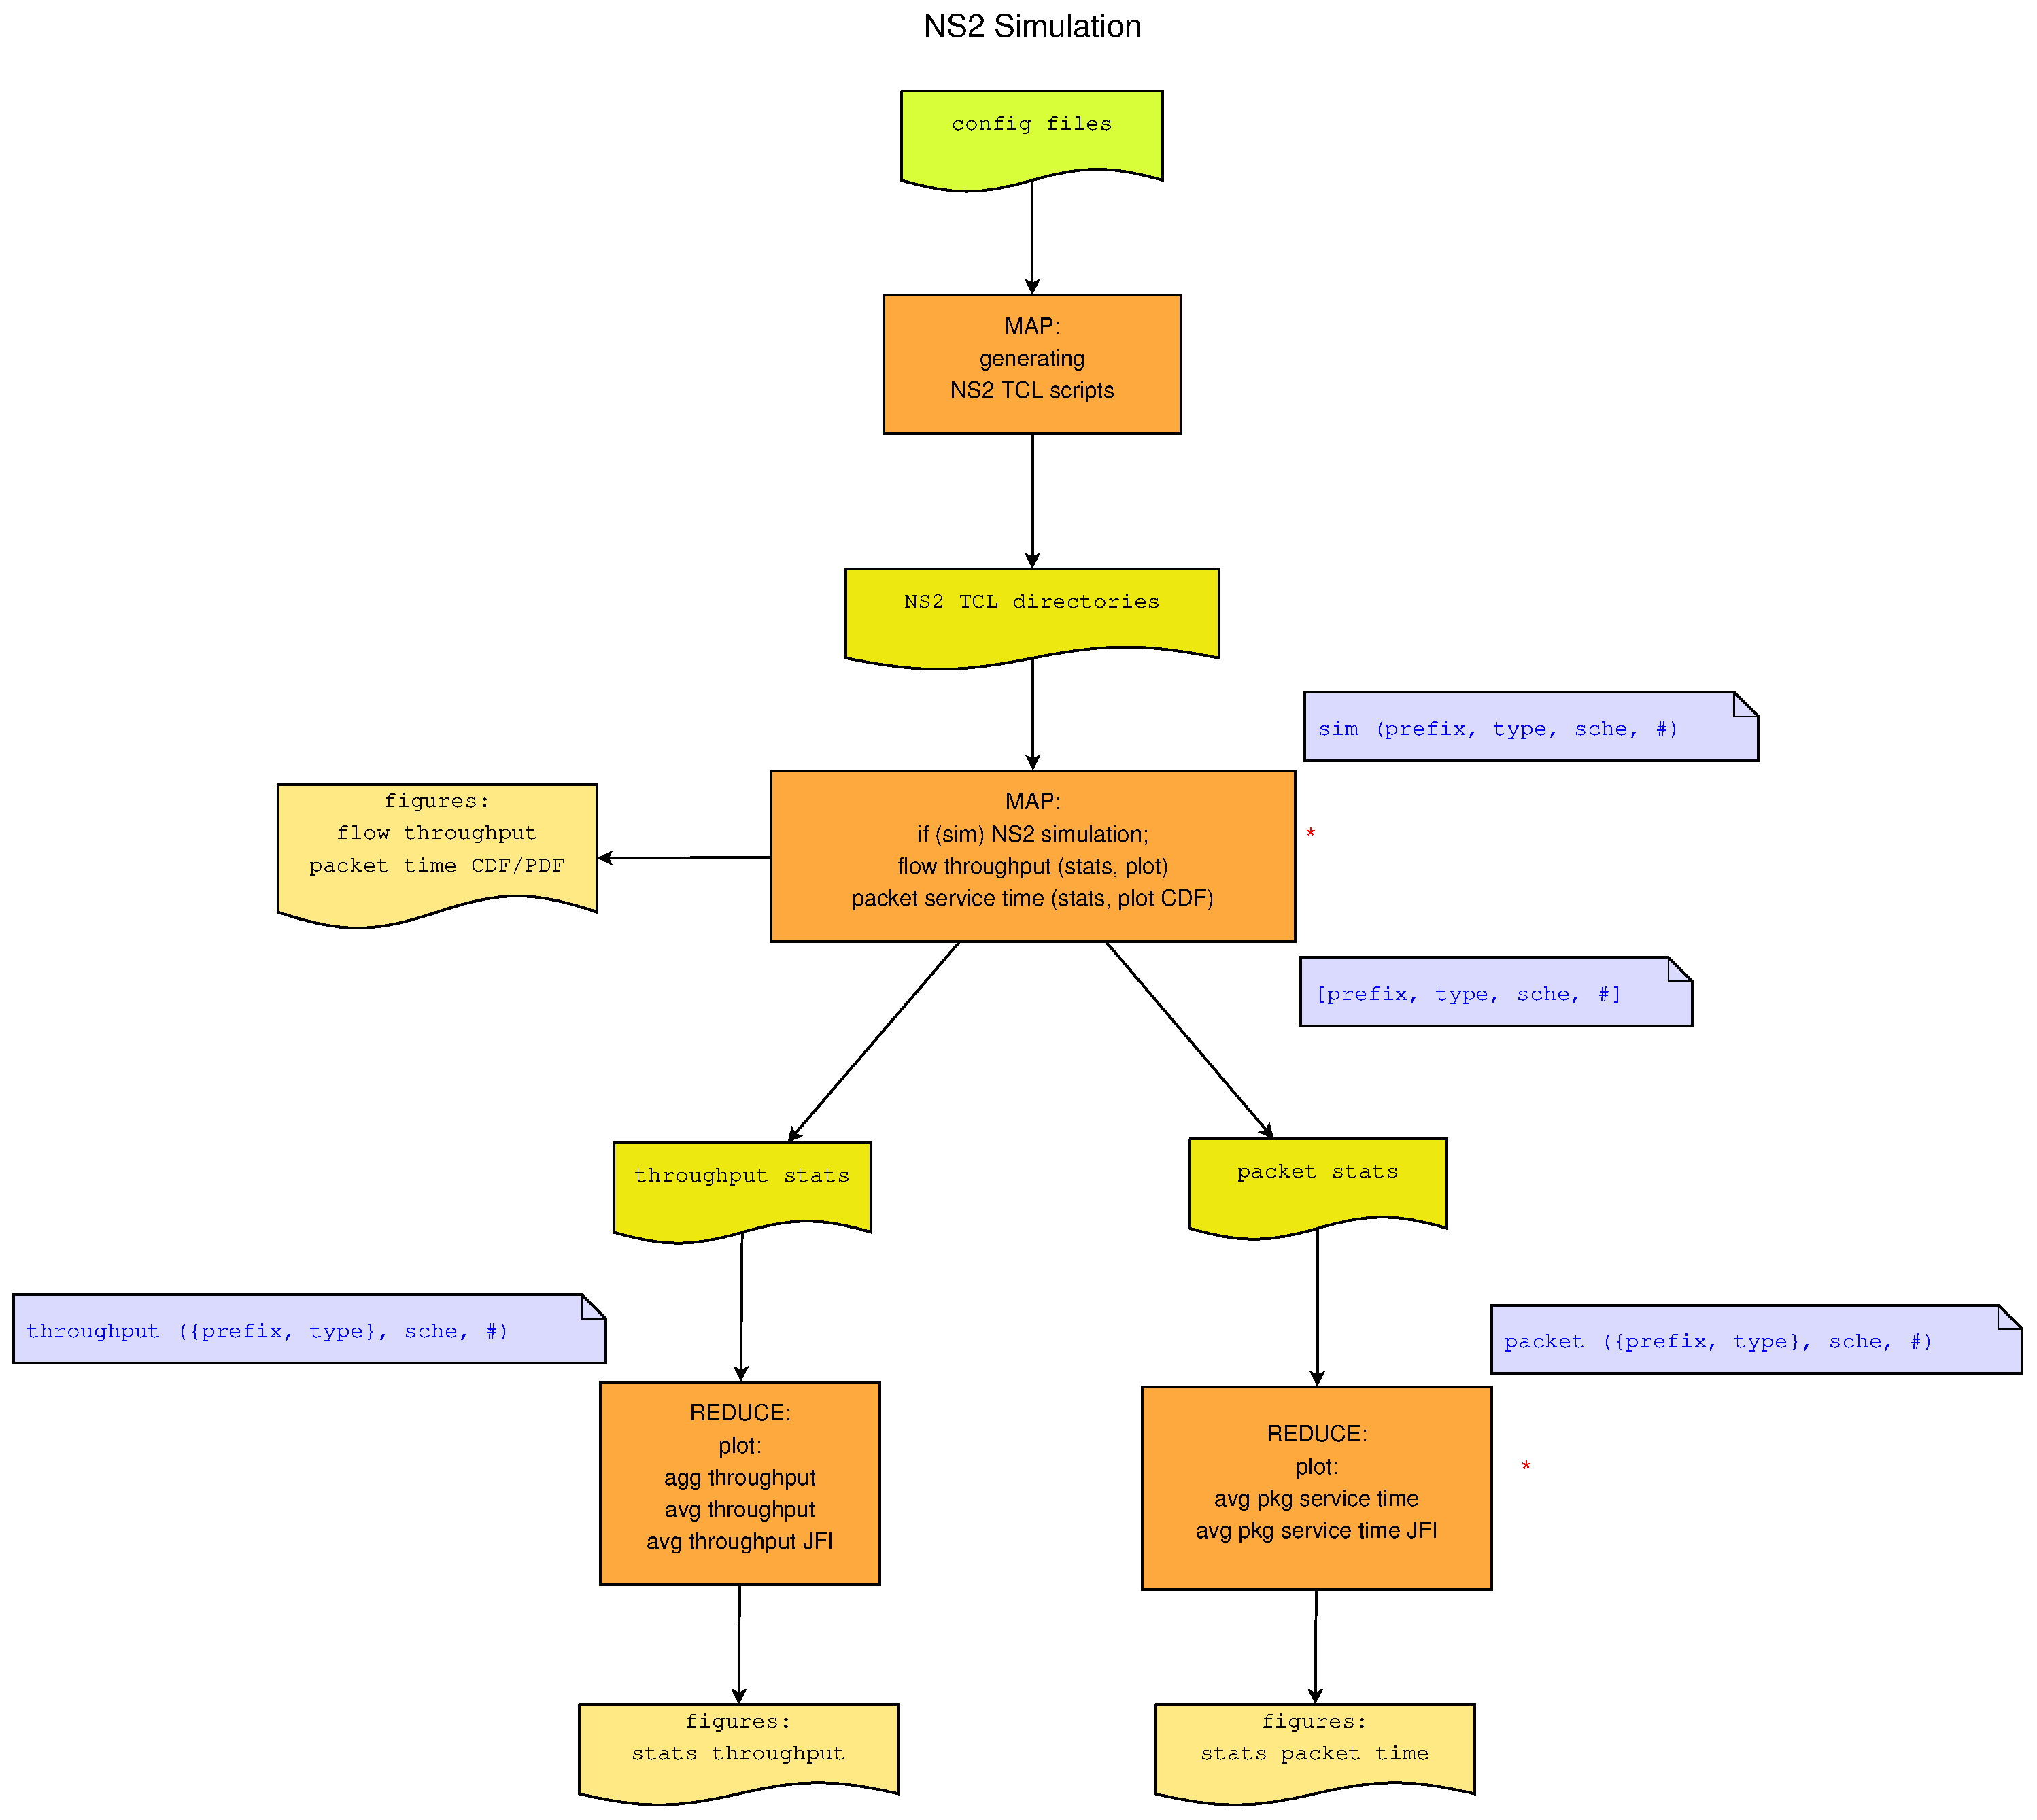
\includegraphics[width=0.9\textwidth]{flowchart-1-ns2figures}
  \caption{The system.
    The text in \fcolorbox{black}{vidtransoriginfile}{this color} is the original input file.
    The text in \fcolorbox{black}{vidtranstmpfile}{this color} is the temp file.
    The text in \fcolorbox{black}{vidtransfinalfile}{this color} is the final output file.
    The text in \fcolorbox{black}{vidtransprocess}{this color} is process block.
    The text in \fcolorbox{black}{vidtransfuncio}{\textcolor[HTML]{0000FF}{this color}} is the input/output of one process block.
The process blocks signed by a \textcolor[HTML]{FF0000}{*} are the blocks cost most of the processing time.
  }\label{fig:system}
\end{figure}

The packet delay time processing includes:
\begin{itemize}
  \item (Mgn) filter out CMTS management packets and stats
  \item (DS) filter out CMTS--CM flow and stats
  \item (US) filter out CM-CMTS flow and stats
  \item Plot DS CDF/PDF
  \item Plot Managment CDF/PDF
\end{itemize}


\chapter{Low Level Design}


\subsection{Interface of the generating configurations}

Use the streaming mode of Map-Reduce.

The input should be the config file list.


\subsubsection{map}
Function: generate directories and move and modify TCL scripts for the test.


Input parameters:
\begin{lstlisting}[language=bash]
<command> <config_file>
# config "/path/to/config.sh"
# config "/path/to/config-jjmbase.sh"
\end{lstlisting}


Output:
\begin{lstlisting}[language=bash]
<command> <config_file> <prefix> <type> <scheduler> <number_of_node>
sim <config_file> <prefix> <type> <scheduler> <number_of_node>
# sim  "jjmbase"  "tcp" "PF" 24
\end{lstlisting}

There should exist the directory contains the TCL scripts and data files for the simulation.





\subsection{Interface of simulation}

This stage will run the simulation base on each directory configuration,
and also generate the related throughput figures.


\subsubsection{map}
Function: run the simulations.


Input parameters:
\begin{lstlisting}[language=bash]
<command> <config_file> <prefix> <type> <scheduler> <number_of_node>
sim <config_file> <prefix> <type> <scheduler> <number_of_node>
# sim "config-xx.sh" "jjmbase"  "tcp" "PF" 24
\end{lstlisting}


Output:
\begin{lstlisting}[language=bash]
<command> <flow_type> <config_file> <prefix> <type> <scheduler> <number_of_node>
throughput <flow_type> <config_file> <prefix> <type> <scheduler> <number_of_node>
packet <flow_type> <config_file> <prefix> <type> <scheduler> <number_of_node>
# throughput "tcp" "config-xx.sh" "jjmbase"  "tcp" "PF" 24
# packet "tcp" "config-xx.sh" "jjmbase"  "tcp+has" "PF" 24
\end{lstlisting}

The routine should run ns2 and process stats, figures of throughput/packet.




\subsubsection{reduce}
Function: plot JFI figures


Input: (all of the columns are keys)
\begin{lstlisting}[language=bash]
<command> <flow_type> <config_file> <prefix> <type> <scheduler> <number_of_node>
throughput <flow_type> <config_file> <prefix> <type> <scheduler> <number_of_node>
packet <flow_type> <config_file> <prefix> <type> <scheduler> <number_of_node>
# throughput "tcp" "config-xx.sh" "jjmbase"  "tcp" "PF" 24
# packet "tcp" "config-xx.sh" "jjmbase"  "tcp+has" "PF" 24
\end{lstlisting}

Output: figures

